\documentclass[11pt,final]{article}

\usepackage[a4paper,margin=1in]{geometry}
\usepackage{amsmath,amssymb}
\usepackage{graphicx}
\graphicspath{{figures/}{../../figures/}}
\usepackage[numbers,sort&compress]{natbib}
\usepackage{xurl}
\usepackage[hidelinks]{hyperref}
\newcommand{\doi}[1]{\href{https://doi.org/#1}{doi:\nolinkurl{#1}}}
\usepackage{float}
\usepackage{microtype}

\title{A Structural Horizon Transition in a Representative TIG Geometry:\\
A Test Against Quadratic $f(R)$ Gravity}

\author{Kai Stefan Dietrich\\
Independent Research}

\date{Revised draft -- wave 4, 2 October 2026}

\begin{document}

\maketitle

\begin{abstract}
We analyze the horizon structure of a specified static, spherically symmetric
representative geometry within the Topological Integrity Gravity (TIG) research
program. The chosen regular mass profile yields the exact dimensionless horizon
equation \(x^3-x^2+\beta^3=0\). We derive its discriminant, positive-root sectors,
and critical point \(x_c=2/3\), \(\beta_c=(4/27)^{1/3}\). The two positive roots
coalesce in a nondegenerate local fold with square-root separation. The cubic
is a consequence of the chosen mass profile, not a universal requirement of
fold bifurcations or dimensional consistency. A direct trace test also excludes
this nontrivial representative metric as an exact vacuum solution of
constant-coefficient quadratic metric \(f(R)\) gravity. This geometry is a reparameterized Hayward metric.
The Schwarzschild limit and bounded-curvature core remain geometric properties.
A prescribed reflecting model yields a conditional inverse-square-root
round-trip delay on the horizonless side. Physical reflection, dynamical
completion and observational forecasts remain separate tasks.
\end{abstract}

\section{Introduction}

General Relativity provides an accurate description of gravitational phenomena across a wide range of scales \cite{einstein1915,wald1984}. Extensions such as $f(R)$ gravity introduce higher-curvature corrections and additional degrees of freedom \cite{sotiriou2010,defelice2010}.

The number of positive horizon roots can depend on a control parameter and change at a critical coalescence. This parameter-dependent root structure is the subject of the present static analysis.

We analyze a specified representative metric and test its compatibility with
quadratic metric $f(R)$ gravity. The algebraic horizon transition is established
for that metric, while the direct vacuum test gives a negative result. Counting
static Killing-horizon roots does not establish dynamical horizon formation.

\section{Consistency Constraint and Model Choice}

Structural consistency and the Schwarzschild limit constrain a model without
uniquely specifying its mass profile or the degree of its horizon equation.
A local fold equilibrium equation is quadratic, $y^2-\lambda=0$; a cubic
potential can generate it by differentiation \cite{chasnov2020}.
Indeed, $x^2-x+\lambda=0$ has a root $x=1$ at $\lambda=0$ and a fold at
$(x,\lambda)=(1/2,1/4)$. Lower-order equations therefore can capture fold
behavior. The cubic below follows specifically from the selected regular
mass profile, rather than from a universal bifurcation requirement.

\section{Quadratic Gravity as a Consistency Test}

We use the metric formalism, signature $(-,+,+,+)$, and geometrized units
$G=c=1$. To retain the convention $\mu=16\pi\alpha$, the action is
\begin{equation}
S=\int d^4x\sqrt{-g}
\left[\frac{R-2\Lambda}{16\pi}+\alpha R^2\right]+S_{\mathrm{matter}}
=\frac{1}{16\pi}\int d^4x\sqrt{-g}\,f(R)+S_{\mathrm{matter}},
\end{equation}
where
\begin{equation}
f(R)=R-2\Lambda+\mu R^2,\qquad \mu=16\pi\alpha.
\end{equation}
Thus $\alpha$ here is the coefficient outside the Einstein prefactor. If the
entire expression $R-2\Lambda+\alpha_{\mathrm{in}}R^2$ were placed inside
that prefactor, its coefficient would instead satisfy $\mu=\alpha_{\mathrm{in}}$.
These are different parameter conventions, not simultaneous definitions of
the same $\alpha$. Here $[\mu]=[\alpha]=L^2$, $[R]=[\Lambda]=L^{-2}$.

The metric field equations are \cite{sotiriou2010,defelice2010}
\begin{equation}
f_R R_{\mu\nu}-\frac{1}{2}f g_{\mu\nu}
 +(g_{\mu\nu}\Box-\nabla_\mu\nabla_\nu)f_R=8\pi T_{\mu\nu},
\end{equation}
with $f_R=1+2\mu R$. Their trace is
\begin{equation}
6\mu\Box R-R+4\Lambda=8\pi T.
\label{eq:fr_trace}
\end{equation}
Linearization about a constant-curvature vacuum background yields
$m_\phi^2=1/(6\mu)$ for the scalar curvature mode. Positive $\mu$ gives a
positive squared mass; this alone is not a proof of full background stability.
The scalar variable $\phi=f_R$ is not assumed to be a canonically normalized
Einstein-frame scalar. No relation between $\mu$ and the core scale $r_c$ follows
from this action comparison.

\section{Effective Geometry}

We consider a static, spherically symmetric metric
\begin{equation}
ds^2=-F(r)dt^2+\frac{dr^2}{F(r)}+r^2d\Omega^2.
\end{equation}

For $M>0$ and $r_c>0$, we choose the representative effective mass profile
\begin{equation}
m(r)=\frac{Mr^3}{r^3+r_c^3},
\end{equation}

leading to
\begin{equation}
F(r)=1-\frac{2m(r)}{r}.
\end{equation}


The asymptotic Schwarzschild limit and the regular-core behavior do not select
this profile uniquely: $\widetilde m(r)=Mr^3/(r^2+r_c^2)^{3/2}$ satisfies both
requirements and gives a different horizon equation. The following calculations
refer only to the specified profile.

For $r_c^3=2M\ell^2$ this is precisely Hayward's static metric
\cite{hayward2006}; its metric and horizon coalescence are not new geometric
discoveries. A fixed-$r_c$ scan is not the fixed-$\ell$ mass evolution of that
dynamical example.

\section{Vacuum Field-Equation Test}

Set $a=r_c^3$. A direct curvature calculation for the stated metric gives
\begin{equation}
R(r)=\frac{12Ma(2a-r^3)}{(r^3+a)^3},\qquad
\Box R=\frac{1}{r^2}\frac{d}{dr}\left(r^2F\frac{dR}{dr}\right).
\end{equation}
In vacuum, Eq.~\eqref{eq:fr_trace} must vanish identically. At infinity its
left side tends to $4\Lambda$, forcing $\Lambda=0$. For that value,
\begin{equation}
\lim_{r\to\infty}r^6(6\mu\Box R-R)=12Ma\ne0,
\qquad
\lim_{r\to0^+}(6\mu\Box R-R)=-\frac{24M}{a}\ne0.
\end{equation}
Therefore this nontrivial representative geometry is not an exact vacuum
solution of constant-coefficient quadratic metric $f(R)$ gravity.
This exclusion does not cover different metric ansatzes or specified matter
models. With matter, its stress tensor and its own equations must be supplied;
defining $T_{\mu\nu}$ from the metric residual alone does not demonstrate that
completion. The Schwarzschild limit $r_c=0$ at $r>0$ is a separate vacuum case.

\section{Critical Horizon Structure}

Candidate static Killing horizons at positive radii satisfy
\begin{equation}
F(r_H)=0.
\end{equation}

This yields
\begin{equation}
r_H^3-2Mr_H^2+r_c^3=0.
\end{equation}

Introducing
\begin{equation}
x=\frac{r_H}{2M}, \qquad \beta=\frac{r_c}{2M},
\end{equation}

the parameter $\beta$ is the dimensionless ratio between the internal scale $r_c$ and the gravitational radius $2M$. It measures the strength of regularization at the horizon scale.

We obtain
\begin{equation}
P(x,\beta)=x^3-x^2+\beta^3=0.
\end{equation}
Here $F=P/(x^3+\beta^3)$; the denominator is positive for $x>0$, $\beta>0$.
At $\beta=0$, the double zero $x=0$ in the cleared polynomial is outside this
equivalence domain and is not a Schwarzschild horizon. The cubic term
$\beta^3$ originates in $r_c^3$ in the chosen mass profile; dimensionlessness
alone does not require it.

The critical value is
\begin{equation}
\beta_c=\left(\frac{4}{27}\right)^{1/3}.
\end{equation}

At criticality, $P=(x-2/3)^2(x+1/3)$. For $0<\beta<\beta_c$ there are two
positive roots and one negative root; at $\beta_c$ one positive double root;
above $\beta_c$ the only real root is negative. The discriminant is
$\Delta=\beta^3(4-27\beta^3)$. Figure~\ref{fig:horizon} illustrates the approach
of the outer branch to the analytically derived critical value. The positive branch count changes,
while the branch locations remain continuous up to coalescence.

\begin{figure}[H]
\centering
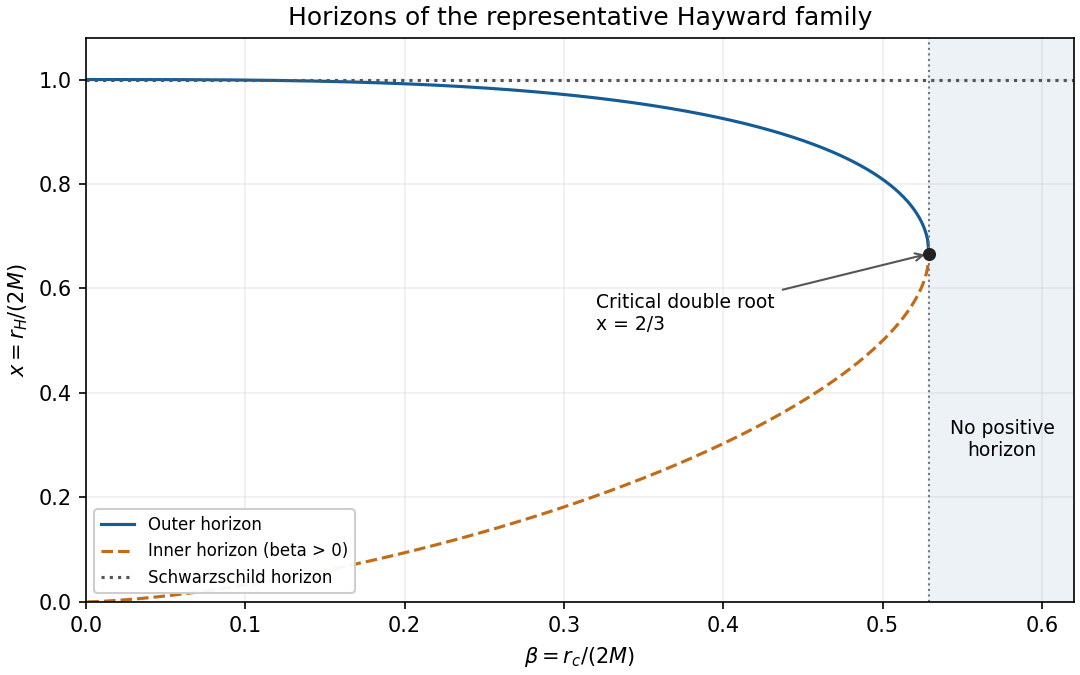
\includegraphics[width=0.75\textwidth]{tig_horizon_branches.png}
\caption{Positive horizon branches of the specified representative Hayward family, obtained from $x^3-x^2+\beta^3=0$. The positive branches merge at $x_c=2/3$ and $\beta_c=(4/27)^{1/3}$. This static parameter diagram does not demonstrate dynamical horizon formation.}
\label{fig:horizon}
\end{figure}

\section{Local Horizon Scaling}

The horizon equation is
\begin{equation}
f(x,\beta)=x^3-x^2+\beta^3=0.
\end{equation}

The critical point is
\begin{equation}
x_c=\frac{2}{3}, \qquad \beta_c=\left(\frac{4}{27}\right)^{1/3}.
\end{equation}

Expanding around criticality yields
\begin{equation}
x_\pm-x_c=\pm\sqrt{3}\,\beta_c\epsilon^{1/2}+O(\epsilon),
\qquad \epsilon=\beta_c-\beta>0.
\end{equation}

The derivatives $P_{xx}(x_c,\beta_c)=2$ and
$P_\beta(x_c,\beta_c)=3\beta_c^2$ are nonzero, so this is a nondegenerate
local fold. The exact expansion is
\begin{equation}
P(x_c+\delta,\beta_c-\epsilon)=\delta^2+\delta^3
-3\beta_c^2\epsilon+3\beta_c\epsilon^2-\epsilon^3.
\end{equation}
Thus the horizon-root displacement exponent in this parameterization is
\begin{equation}
\alpha_H=\frac{1}{2}.
\end{equation}

\section{Literature Context and Theorem Boundaries}

Static horizon roots and dynamical formation are distinct. Hayward's
time-dependent example supplies mass evolution and fluxes
\cite{hayward2006}; these are additional inputs, not consequences of our cubic.
Trapping horizons need not be global event horizons.

The zeroth-law analysis of Ghosh and Sarkar \cite{ghosh2026zerothlaw}
assumes a smooth stationary Killing horizon and appropriate field equations
and matter conditions. Its Ricci-squared argument uses nonzero coupling,
a compact connected boundaryless section and non-extremality. Pure $f(R)$
uses the mixed projection and requires $f_R\ne0$ instead.
Our critical horizon has $\kappa=0$; spherical angular constancy does not
prove a field-equation solution or horizon formation.

Bessa \cite{bessa2026matterdensityquadratic} studies scalar dust perturbations
of flat FLRW in full quadratic gravity, including Weyl squared, with
sub-horizon and quasi-static approximations. Its formal infrared continuation
does not prove TIG perturbative stability or a controlled super-horizon limit.

Garay et al.\ \cite{garay2026globalvariablesemergentcosmology} provide an
indirect two-vertex LQG comparison, not ordinary quantum mechanics recovered
from TIG. Finite-dimensional quantum reconstruction
\cite{chiribella2011} requires its own operational assumptions.
No TIG derivation of these assumptions or quantum recovery is supplied here.

\section{Conditional Round-Trip Delay}

In a connected static region with $F>0$, radial null propagation gives
$dt=\pm dr/F$. We additionally prescribe an inner reflector at
$r_{\rm ref}=2Mx_{\rm ref}>0$ and a partially reflecting, transmitting outer
scattering boundary at $r_b=2Mx_b$. Neither boundary is derived from TIG.
The geometric round-trip time in asymptotically normalized $t$ is
\begin{equation}
T_{\rm rt}=2\int_{r_{\rm ref}}^{r_b}\frac{dr}{F}
=4M\int_{x_{\rm ref}}^{x_b}\frac{x^3+\beta^3}{x^3-x^2+\beta^3}\,dx.
\label{eq:roundtrip}
\end{equation}
Echo-like output additionally requires excitation and appropriate scattering;
this formula supplies neither a waveform nor a gravitational perturbation
equation. A minimally coupled massless test scalar would have
\begin{equation}
(-\partial_t^2+\partial_{r_*}^2-V_\ell)\psi_\ell=0,\qquad
\frac{dr_*}{dr}=\frac1F,\qquad
V_\ell=F\left[\frac{\ell(\ell+1)}{r^2}+\frac{F'}r\right].
\end{equation}
An ideal Dirichlet inner boundary reflects that test field; its physical
origin and the required outer scattering remain assumptions.
The horizonless-object calculation of Cardoso et al.\ \cite{cardoso2016}
is a methodological comparison with different geometry and boundary data.
Its one-way delay is distinct from the round trip defined here.

For fixed $M$, set $\eta=\beta-\beta_c>0$, $\delta=x-x_c$,
$D_0=4/9$ and $s=\sqrt3\beta_c\sqrt{\eta}$. Above criticality $F>0$ at
all positive radii. The exact numerator is
\begin{equation}
P=\delta^2+\delta^3+3\beta_c^2\eta+3\beta_c\eta^2+\eta^3.
\end{equation}
Its bottleneck has $F\sim(\delta^2+s^2)/D_0$. If the fixed endpoints
satisfy $0<x_{\rm ref}<x_c<x_b$, the scaled integral in
Eq.~\eqref{eq:roundtrip} contains
$\int_{-\infty}^{\infty}dy/(1+y^2)=\pi$ and hence
\begin{equation}
T_{\rm rt}\sim\frac{16\pi M}{9\sqrt3\beta_c}
(\beta-\beta_c)^{-1/2},\qquad \beta\downarrow\beta_c,\quad\beta>\beta_c.
\label{eq:conditional_delay}
\end{equation}
The ratio to this leading term tends to one. The local scaled integrand is
dominated by a constant times $(1+y^2)^{-1}$; regions away from $x_c$
have bounded travel time. One fixed endpoint at $x_c$ halves the coefficient;
two fixed endpoints strictly on the same side have a finite limit.
A fixed exterior observer with a finite positive limiting lapse measures
$\Delta\tau_{\rm obs}=\sqrt{F(r_{\rm obs})}\,T_{\rm rt}$.

Below criticality, let $\epsilon=\beta_c-\beta>0$ and
$s=\sqrt3\beta_c\sqrt{\epsilon}$. Returning exterior paths must stay at
$x>x_+$. Fixed $x_c<x_{\rm ref}<x_b$ give a finite critical limit.
Only the additional tracking prescription
$x_{\rm ref}=x_++(q-1)s$, with fixed $q>1$, gives
\begin{equation}
T_{\rm rt}\sim\frac{2MD_0}{\sqrt3\beta_c}
\ln\frac{q+1}{q-1}\,\epsilon^{-1/2}.
\end{equation}
This prescribes a coordinate gap, not a fixed proper gap.
At fixed subcritical $\beta$, a mirror approaching the simple outer horizon
instead gives $T_{\rm rt}=-\kappa_+^{-1}\ln(h/L)+O(1)$, where
$h=r_{\rm ref}-r_+\to0^+$ and $L>0$ is fixed.
At exact criticality, $x_{\rm ref}=x_c+d$ gives
$T_{\rm rt}\sim16M/(9d)$ as $d\to0^+$.
Crossing a future outer horizon is not a returning exterior signal path.
The former unrestricted $(\beta_c-\beta)^{-1/2}$ echo claim therefore does
not hold for arbitrary boundaries. Equation~\eqref{eq:conditional_delay}
is a conditional geometric delay, not a demonstrated physical TIG echo.

\section{Conclusion}

The specified representative TIG geometry has an exact cubic horizon equation
and a nondegenerate fold with horizon-root exponent $1/2$. Neither structural
consistency nor a generic fold uniquely requires this cubic mass-profile law.
The nontrivial metric fails the vacuum trace equation of the tested quadratic
metric $f(R)$ action; no exact solution with specified matter has been
demonstrated. The algebraic horizon result remains model-conditional, while
dynamical completion, stability, and echo forecasts require separate evidence.


The static family is identified with Hayward's earlier metric. With additionally
prescribed reflection and fixed endpoints straddling the horizonless bottleneck,
the round-trip delay has exponent $-1/2$ on the $\beta>\beta_c$ side.
Subcritical delays depend on the mirror prescription. Neither this kinematic
calculation nor the comparison literature establishes physical TIG echoes,
dynamical horizon formation or quantum-mechanical recovery.

\begingroup
\small
\setlength{\bibsep}{4pt}
\bibliographystyle{unsrtnat}
\bibliography{references}
\endgroup

\end{document}
